%%%--------------------------------%%%
%%% Implementation
%%%--------------------------------%%%
\section{General Infrastructure}
\label{sec:implementationInfra}

The implementation of the use cases Project Access Management (\ref{sec:domainBbc}) and User CRUD (\ref{sec:domainBbb}) is finished at the time of this paper's submission. According to the use cases, users can create an account and then be invited to projects or create them themselves. Both use cases had to be implemented beforehand as risks should be related to a project which again are composed of multiple users (\ref{sec:domainBbc}, \ref{sec:domainBbb}).

\begin{wrapfigure}{r}{0.5\textwidth}
	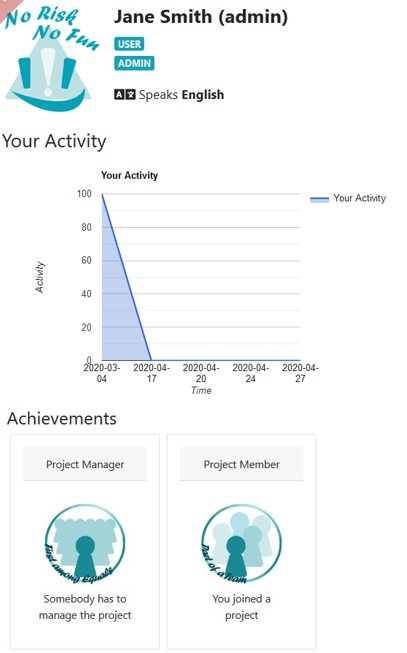
\includegraphics[width=0.5\textwidth]{Assets/implementation_shots/profile.png}
	\caption{Screenshot of finalization step}
	\label{fig:ShotProfile}
\end{wrapfigure}


In figure \ref{fig:ShotProfile} one can see the profile page of a user which is available after logging in. Additionally, one part of the gamification elements is visible: user achievements which can be acquired by different actions such as being responsible for a project risk.



Figure \ref{fig:ShotProjectCreation} shows the creation dialog for a project. After entering the necessary information and submitting by clicking “Save”, the project is created and will be available for all its members. This information can be edited later. The same applies to the information for the user/personal account which can be edited in separate view. Within a project, a member can create and discuss project risks (\ref{sec:implementationRisks}), which the following section elaborates on further.

\begin{figure}[H]
	\centering
	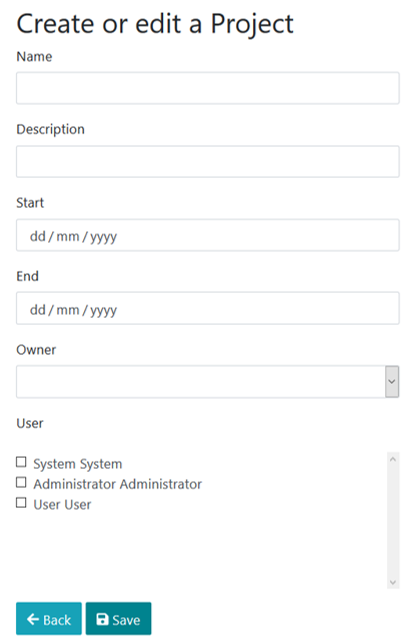
\includegraphics[width=0.5\textwidth]{Assets/implementation_shots/CreateProject.png}
	\caption{Screenshot of project cration page}
	\label{fig:ShotProjectCreation}
\end{figure}

